\documentclass[10pt, a4paper, spanish]{article}
\usepackage[paper=a4paper, left=1.5cm, right=1.5cm, bottom=1.5cm, top=3.5cm]{geometry}
\usepackage[utf8]{inputenc}
\usepackage[spanish]{babel}
\usepackage{caratula}
\usepackage{aed2-symb,aed2-itef,aed2-tad,aed2-dis,caratula}
\usepackage[pdfencoding=auto, colorlinks=true, linkcolor=blue]{hyperref}
\usepackage[boxruled, longend]{algorithm2e}
\usepackage{wrapfig}
\usepackage{tikz}
\usetikzlibrary{babel}

\tikzset{nodeList/.style={every node/.style={draw, circle}}}
\tikzset{pathList/.style={every node/.style={midway, fill=white}}}

\begin{document}

% CARATULA
\materia{Algoritmos y Estructuras de Datos III}
\submateria{Primer Cuatrimestre de 2017}
\fecha{\today}
\grupo{Grupo ``Dijkstraidos''}
\titulo{Trabajo Práctico 3}

\integrante{Barylko, Roni Ariel}{750/15}{rbarylko@dc.uba.ar}
\integrante{Giudice, Carlos}{694/15}{cgiudice@dc.uba.ar}
\integrante{Szperling, Sebastián Ariel}{763/15}{sszperling@dc.uba.ar}
\integrante{Tarrío, Ignacio}{363/15}{itarrio@dc.uba.ar}

\maketitle

\tableofcontents

\pagebreak


\section{Descripcion de situaciones reales}
El problema que vamos a analizar durante todo el informe es el de \textit{clique de máxima frontera}(\textit{CMF}) en un grafo, que consiste en hallar la clique tal que su frontera sea de cardinalidad máxima. Definimos la frontera de una clique K como el conjunto de aristas que tienen un extremo en K y otro por fuera de la clique.

Distintas situaciones problemáticas de la vida real podrían ser representadas por CMF, tales como:

\begin{itemize}

\item MarencoGames desarrolla un juego online y quiere que haya la menor cantidad de gente haciendo trampa. En este juego los jugadores juegan a través de la red, pero no todos están comunicados entre sí. Los desarrolladores quieren hacer un sistema de protección de trampa, por lo que deciden convertir varios jugadores en moderadores, los cuales van a reportar cuales de los participantes a los que están conectados están haciendo trampa. Los moderadores tienen que estar todos conectados entre sí para reportarse las trampas, y lo que se desea es cubrir la mayor cantidad de jugadores posibles.  Cada jugador puede ser representado con un nodo, y la conexión entre dos jugadores a través de aristas. Con esta representación, tendríamos que una clique en el grafo podrá ser un conjunto de moderadores conectados entre sí, y la frontera será la cantidad de jugadores que abarca el sistema de protección.

\item En un proyecto en conjunto llevado a cabo por alumnos de Biología y Computación, se quiere desarrollar un robot que tenga un comportamiento similar al de las arañas. Para esto, los biólogos realizaron una investigación y llegaron a la conclusión de que los arácnidos, a la hora de situarse en sus telarañas, buscan cumplir dos requisitos: mantenerse seguras, y alcanzar sus presas con total rapidez. De este modo, a los computólogos se les ocurrió imaginar la telaraña como un grafo, donde cada hilo será una arista y cada intersección un vértice. De este modo, como son los hilos los que protegen a la araña, un lugar seguro será aquel donde todos los vértices tengan un hilo entre sí, y un sitio alcanzable será todo vértice que se encuentre relacionado a un hilo que llegue hacia donde esta ella. Nuestra araña, de manera instintiva, no permitirá que ninguna presa se acerce adonde esta situada, por lo que solo consideraremos los sitios alcanzables por afuera de su lugar seguro. Como los alumnos concluyeron que sería más divertido tener una araña violenta, optaron por configurarla de manera que priorice el alcance a las presas antes que la seguridad, de modo que busque la posición segura donde más sitios alcanzables haya.

%TODO poner varios problemas mas

\end{itemize}



\pagebreak
\section{Algoritmo exacto}


\section{Metaheurística GRASP}
	\subsection{Desarrollo}
Hemos propuesto dos métodos que computan una solución, formulándola en base a criterios heurísticos. La limitación de los enfoques anteriores reside en que se recorre el espacio de soluciones hasta que no es posible mejorar la solución. Como sabemos que una solución maximal no necesariamente es máxima, sería útil poder contrastar distintas soluciones maximales y elegir la mejor. En otras palabras, quisiéramos ramificar la exploración del espacio de soluciones, para así aumentar nuestras posibilidades de encontrar la clique de máxima frontera.

Habiendo notado que heurísticas determinísticas siempre toman la misma decisión en el mismo paso, se propone la utilización de una heurística pseudo-greedy. Esta heurística aleatoriamente tomará decisiones localmente buenas pero no necesariamente óptimas. Se considerará que la decisión de agregar un nodo es buena si agregarlo aumenta el tamaño de la frontera. Para tener cierto control sobre que tan goloso es el comportamiento de esta heurística, se puede pedir que la elección aleatoria sea tomada teniendo en cuenta solo el mejor porcentaje de las decisiones posibles (es decir, que se elija aleatoriamente una opción buena dentro del X por ciento más alto). Si el porcentaje es chico, solo se consideraran las mejores opciones y el comportamiento será muy similar a la heurística greedy pura. Esto restringiría la ramificación que buscabamos. Si el porcentaje es muy alto, existirá la posibilidad de agregar un nodo de grado muy bajo a la clique, lo cual restringirá en gran medida la cantidad de nodos que se pueden agregar, obteniendo muy posiblemente una clique pequeña. 


\begin{algorithm}[H]
	\NoCaptionOfAlgo
	\caption{\algoritmo{randomGreedy}{\In{listaAdyacencia}{lista}, \In{float}{porcentajeConsiderado}}{clique}}
	
	nodosConsiderados $\leftarrow$ nodos(lista)
	
	ordenarPorGrado(nodosConsiderados)
	
	indiceNodoAleatorio $\leftarrow$ nodoAleatorio(nodosConsiderados, porcentajeConsiderado)
	
	nodoPorAgregar $\leftarrow$ nodosConsiderados[indiceNodoAleatorio]
	
	agregarNodoAClique(res, nodoPorAgregar)
	
	nodosConsiderados $\leftarrow$ nodoPorAgregar.adyacentes()

	ordenarPorGrado(nodosConsiderados)
	
	res $\leftarrow$ recurRandomGreedy(lista, res, nodosConsiderados, porcentajeConsiderado)


\end{algorithm}

\begin{algorithm}[H]
	\NoCaptionOfAlgo
	\caption{\algoritmo{recurRandomGreedy}{\In{listaAdyacencia}{lista}, \In{clique}{cliqueParcial}, \In{listaNodos}{nodosConsiderados}\In{float}{porcentajeConsiderado}}{clique}}
	
	\If{nodosConsiderados.size() $=$ 0}
	{
		return cliqueParcial
	}
	
	\For{nodo $\in$ nodosConsiderados}
	{
		\If{nodo.grado() $<$ cliqueParcial.size() * 2 $\vee$ nodo.esAdyacenteATodos(clique, lista)}
		{
			nodosConsiderados.borrar(nodo)
		}
	}

	\If{nodosConsiderados.size() $=$ 0}
	{
		return cliqueParcial
	}
	
	indiceNodoAleatorio $\leftarrow$ nodoAleatorio(nodosConsiderados, porcentajeConsiderado)
	
	nodoPorAgregar $\leftarrow$ nodosConsiderados[indiceNodoAleatorio]
	
	agregarNodoAClique(res, nodoPorAgregar)

	nodosConsiderados.borrar(nodoPorAgregar)
	
	res $\leftarrow$ recurRandomGreedy(lista, cliqueParcial, nodosConsiderados, porcentajeConsiderado)

\end{algorithm}

\begin{algorithm}[H]
	\NoCaptionOfAlgo
	\caption{\algoritmo{nodoAleatorio}{\In{listaNodos}{nodosConsiderados}\In{float}{porcentajeConsiderado}}{clique}}
	
		cantidadPorConsiderar $\leftarrow$ nodosConsiderados.size() $*$ (1 - porcentajeConsiderado)
		
		res $\leftarrow$ random(rango(cantidadPorConsiderar))

\end{algorithm}

Cada vez que se elige un nodo, se hace eligiendo aleatoriamente uno que esté entre los mejores de la lista de nodos agregables. En un principio, todos los nodos son elegibles para formar una clique trivial de tamaño uno. El criterio utilizado para elegir alguno es la priorización de nodos de grado alto. Es por esto que en primer lugar se ordenan los nodos en base a su grado y, luego, se elige uno aleatoriamente entre los primeros. El porcentaje a considerar es una variable de entrada que determinará el comportamiento de la heurística.

La función recursiva tiene un procesamiento muy similar, pero toma como parámetro a una clique y una lista de nodos a considerar. En el caso base, si no quedan nodos por considerar, la clique es maximal. Sino, toma la lista y le filtra los nodos que no son adyacentes a todos los nodos de la clique o que no agrandarían la frontera por tener un grado muy chico. Vuelve a preguntar si quedan nodos a considerar y, en caso afirmativo, elige un nodo aleatorio entre los mejores y lo agrega a la clique. Elimina a ese nodo de la lista de nodos a considerar y se llama recursivamente. Como en cada paso la cantidad de nodos a considerar disminuye al menos en una unidad, sabemos que la función eventualmente llega al caso base.

La metaheurística GRASP utiliza tanto búsqueda local como greedy aleatorio. La idea esta en que greedy aleatorio avanza estocásticamente por el espacio de soluciones hasta que llega a una solución maximal. Posteriormente esta solución se pasa como parametro a la búsqueda local. Si hacemos esto muchas veces, tenemos la posibilidad de llegar a muchas soluciones diferentes y así quedarnos con la mejor. Se memoriza la mejor encontrada y en cada iteración del ciclo se compara una nueva solución. Si iteramos lo suficiente, tendremos seguridad de que la solución que guardamos es la mejor entre muchas posibilidades. 

\begin{algorithm}[H]
	\NoCaptionOfAlgo
	\caption{\algoritmo{grasp}{\In{listaAdyacencia}{lista}, \In{unsigned int}{iteraciones}, \In{float}{porcentajeConsiderado}}{clique}}

	bestClique $\leftarrow \emptyset$
	 
	\For{i $\in$ rango(iteraciones)}
	{
		tempClique $\leftarrow$ local(randomGreedy(lista, porcentajeConsiderado))
		 
 		\If{bestClique.frontera() $<$ tempClique.frontera()}
		{
			bestClique $\leftarrow$ tempClique
		}
		 
	}
	
	res $\leftarrow$ bestClique

\end{algorithm}

\subsection{Cota temporal}
La complejidad de randomGreedy está dada por:

\begin{itemize}
    \item \textbf{nodos(lista)}: Devuelve una lista que contiene a todos los nodos del grafo en $O(n)$.

	\item \textbf{ordenarPorGrado}: Esta función utiliza por detrás el sort de la STD, y como lo usamos para ordenar toda la lista de nodos, su complejidad en peor caso es de $O(n*log(n))$.

	\item \textbf{indiceNodoAleatorio}: Devuelve un número aleatorio en $O(1)$.

	\item \textbf{agregarNodoAClique}: Se encarga de actualizar la clique agregando atrás del vector de nodos en la clique el nodo a insertar en $O(1)$.	

\end{itemize}

Con estos costos analizados, y considerando que la función \textbf{esAdyacenteATodos} fue analizada en casos anteriores, podemos pasar a analizar la complejidad de la función recursiva. Dado que esta función termina cuando el parámetro nodosPorConsiderar es de tamaño cero, y que en el peor de los casos puede empezar siendo de tamaño $O(n)$ y decrecer en una unidad en cada llamada recursiva, se concluye que en el peor de los casos se realizarán $O(n)$ llamadas recursivas. En cada una, hay un ciclo de $O(nodosPorConsiderar)$ iteraciones, donde por dentro se llama a la funcion \textbf{esAdyacenteATodos}, que es $O(n)$. Como en el peor de los casos nodosPorConsiderar decrece de a una unidad, la complejidad se reduce a considerar las $n$ llamadas recursivas, que cuentan dentro con un ciclo de $n$ nodos y un algoritmo de complejidad $O(n)$. Por lo tanto, nuestra complejidad acaba siendo $O(n^3)$.

Dado que GRASP esta compuesto por un ciclo que corre tantas veces como se le especifique en el parámetro iteraciones, el costo temporal va a depender linealmente del número de iteraciones. Por otro lado, hay que considerar que en cada iteración del ciclo se realiza una llamada a localSearch(randomGreedy()). Por lo tanto, lo que acaba ocurriendo es que se suman las complejidades de ambos algoritmos (pues Local Search corre solo una vez sobre la clique generada, por lo que su complejidad es ajena a la de randomGreedy). Por ende, el costo de localSearch(randomGreedy()) es $O(n^3)$ + $O((min(n,m))^3$ $\times$ $n^2)$, y como no podemos afirmar nada sobre $min(n,m)$, no podemos realizar ninguna cota. Por lo tanto, nuestra complejidad acaba siendo $O(iteraciones \times (n^3 + min(n,m))^3$ $\times$ $n^2))$.

\subsection{Casos Patológicos}

Ya que la metaheurística tiene un grado de aleatoriedad, es difícil encontrar casos patológicos. Sin embargo, como la misma utiliza internamente las heurísticas de búsqueda local y constructiva golosa, cuyo casos patológicos son parecidos, tendremos en cuenta este tipo de instancias. De cualquier manera, hay que ganarle a la probabilidad que se seleccione algún nodo de los de la clique de la mejor solución. Para evitarlo, hay que disminuir la probabilidad de que seleccione uno de estos nodos, por lo que podemos generar muchas componentes como la de mayor grado para que sea muy probable que, en las iteraciones, seleccione estos nodos en vez de los de la solución máxima. Notemos que podemos generar la cantidad que queramos de este tipo de componentes por lo que mientras más generemos, menos probabilidad tendremos de seleccionar la clique.

\begin{SCfigure}[1][h]
\caption{En la imagen podemos apreciar cómo copiamos 4 veces la componente que tiene el nodo de mayor grado, así estas componentes tienen más probabilidad de ser seleccionadas.}
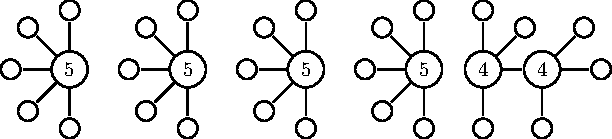
\includegraphics[width=0.5\textwidth]{img/patologicGrasp.pdf}
\end{SCfigure}

\subsection{Experimentación}

Al experimentar con la metaheurística, primero decidimos analizar el impacto lineal de las iteraciones:

\noindent
\begin{minipage}{0.55\textwidth}
    \hfill
    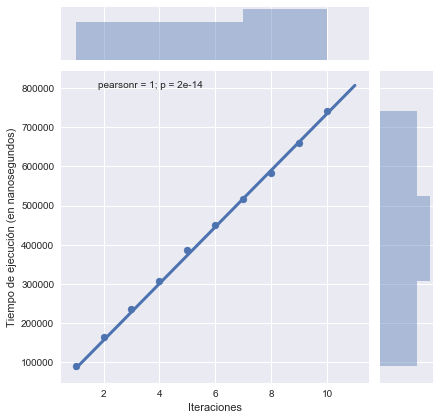
\includegraphics[scale=0.6]{img/grasp-it.png}
\end{minipage}
\hfill
\begin{minipage}{0.44\textwidth}
    \begin{center}
        Datos del gráfico

        \begin{tabular}{ | l l |}
            \hline
             & $n = 10$ \\ 
             & $m =  \frac{n * (n-1)}{2} = 45$ \\ 
            Porcentaje de nodos & \\
            considerados & $p = 0.5$ \\ 
            Curva aproximada & $f(x) = 72500 * x * 10000$ \\
            \hline
        \end{tabular}
    \end{center}
\end{minipage}

Este resultado era más que esperado, ya que resulta de ejecutar las mismas operaciones una cantidad fija de veces. Teniendo esto en cuenta, podemos analizar los demás factores en el caso de una única iteración.

\noindent
\begin{minipage}{0.55\textwidth}
    \hfill
    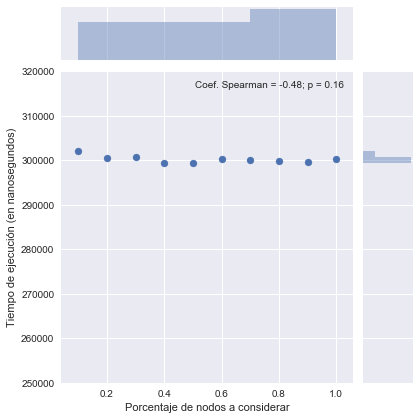
\includegraphics[scale=0.6]{img/grasp-p.png}
\end{minipage}
\hfill
\begin{minipage}{0.44\textwidth}
    \begin{center}
        Datos del gráfico

        \begin{tabular}{ | l l |}
            \hline
             & $n = 10$ \\ 
             & $m =  \frac{n * (n-1)}{2} = 45$ \\ 
            Iteraciones & $it = 1$ \\
            \hline
        \end{tabular}
    \end{center}
\end{minipage}

Dado que los grafos analizados son completos, el porcentaje de nodos a considerar no influye de manera significativa en el tiempo de ejecución. Esto se debe a que la clique máxima es el grafo de entrada en su totalidad. Sin embargo, este porcentaje puede influir en el tiempo de ejecución si el grafo no es uniforme:

\begin{center}
    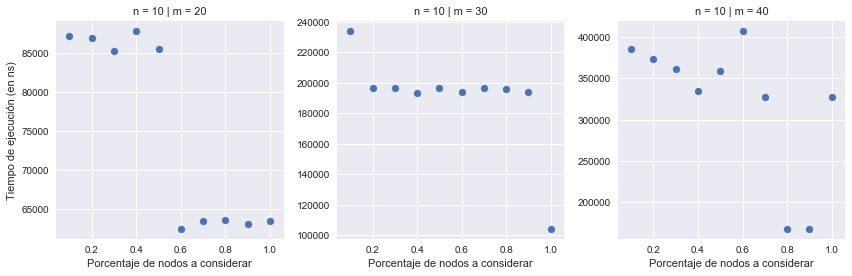
\includegraphics[scale=0.6]{img/grasp-p-multi.png}
\end{center}

La variación en performance se debe en particular a 2 motivos. Por un lado, las búsquedas golosas aleatorias generan una cierta variabilidad en los resultados obtenidos, por lo que resulta difícil determinar qué corresponde a ruido y qué a un camino de decisiones distinto. Por el otro, a medida que aumentamos el porcentaje de los nodos a considerar, permitimos que ciertas instancias ``menos óptimas'' (desde una perspectiva golosa) sean utilizadas, lo cual puede llevar a decisiones no tan útiles y, por ende, cliques más pequeñas. Esto aplica en particular a los grafos con menor cantidad de aristas, ya que mientras más tenga, mayor será en general el grado los nodos, y por consiguiente siempre se considerará agregar más nodos a la clique final.

Una vez analisados estos factores y su impacto, nos dispusimos a medir el tiempo de ejecución en base al tamaño del grafo (utilizando grafos completos una vez más para analizar peor caso):

\noindent
\begin{minipage}{0.55\textwidth}
    \hfill
    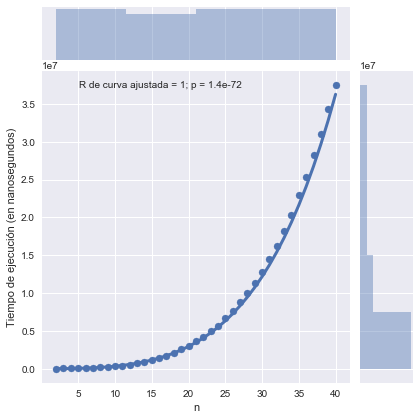
\includegraphics[scale=0.6]{img/grasp-n.png}
\end{minipage}
\hfill
\begin{minipage}{0.44\textwidth}
    \begin{center}
        Datos del gráfico

        \begin{tabular}{ | l l |}
            \hline
            Grafo completo & $m =  \frac{n * (n-1)}{2}$ \\
            Porcentaje de nodos & \\
            considerados & $p = 0.5$ \\
            Iteraciones & $it = 1$ \\
            Curva aproximada & $f(x) = (x^5) / 6 + 300 * x^3$ \\
            \hline
        \end{tabular}
    \end{center}
\end{minipage}

Como se mencionó, la cota de complejidad de GRASP es muy similar a la de una búsqueda local. Por ende, también realizamos gráficos similares a estos, con escala logarítmica y en base a $m$.

\noindent
\begin{minipage}{0.55\textwidth}
    \hfill
    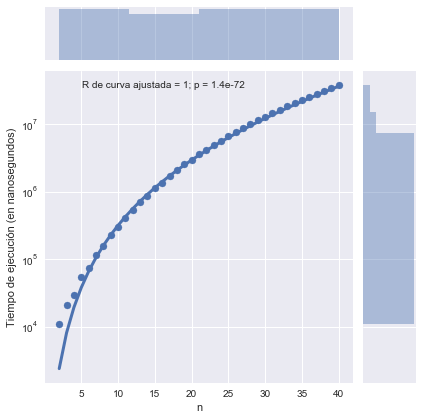
\includegraphics[scale=0.6]{img/grasp-n-log.png}
\end{minipage}
\hfill
\begin{minipage}{0.44\textwidth}
    \begin{center}
        Datos del gráfico

        \begin{tabular}{ | l l |}
            \hline
            Grafo completo & $m = \frac{n * (n-1)}{2}$\\
            Porcentaje de nodos & \\
            considerados & $p = 0.5$ \\
            Iteraciones & $it = 1$ \\
            Curva aproximada & $f(x) = (x^5) / 6 + 300 * x^3$ \\
            \hline
        \end{tabular}
    \end{center}
\end{minipage}

\noindent
\begin{minipage}{0.55\textwidth}
    \hfill
    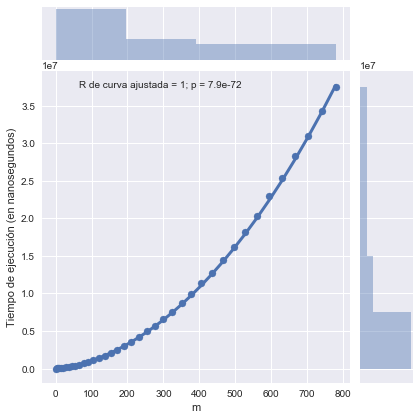
\includegraphics[scale=0.6]{img/grasp-m.png}
\end{minipage}
\hfill
\begin{minipage}{0.44\textwidth}
    \begin{center}
        Datos del gráfico

        \begin{tabular}{ | l l |}
            \hline
            Grafo completo & $m = \frac{n * (n-1)}{2}$\\
            Porcentaje de nodos & \\
            considerados & $p = 0.5$ \\
            Iteraciones & $it = 1$ \\
            Curva aproximada & $f(x) = x^{2.5} + 950 * x^{1.5}$ \\
            \hline
        \end{tabular}
    \end{center}
\end{minipage}

En este caso, parece que la curva propuesta es mucho más precisa que la elegida para la búsqueda local, tanto de forma visual como por el p-valor asociado al coeficiente de Pearson

\subsection{Entrenamiento de la metaheurística}

Además de experimentar con los tiempos de ejecución, decidimos analizar la influencia de ambos parámetros de entrada de la metaheurística en la precisión de los resultados obtenidos. Para esto, utilizamos un conjunto de tests de tamaño moderado, cuyas soluciones fueron obtenidas a través del algoritmo exacto. Para cada caso de prueba, probamos distintos valores para dichos parámetros y comparamos el resultado con el obtenido por fuerza bruta.

A fines prácticos, llamaremos $it$ al número de iteraciones realizadas, y $p$ al porcentaje de nodos a considerar (entre 0 y 1).

\begin{center}
    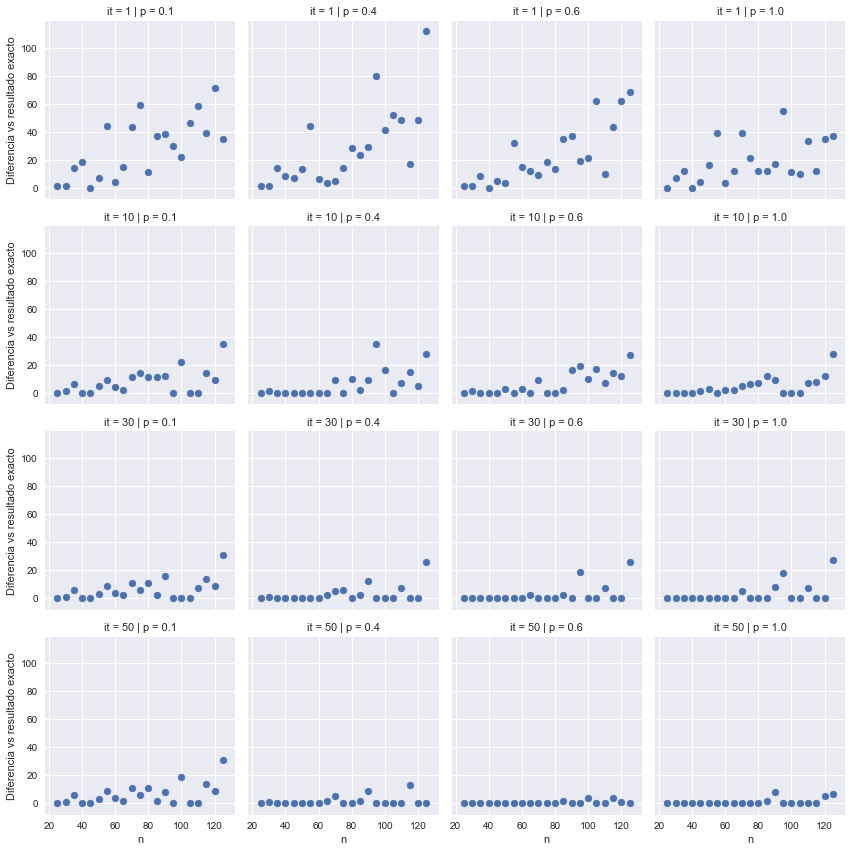
\includegraphics[scale=0.6]{img/grasp-4x4.png}
\end{center}

Este set de resultados nos resultó muy interesante. Pudimos comprobar que, casi siempre, realizar más iteraciones del algoritmo resulta en un resultado mejor (cosa que nos resultaba trivial, aunque podría no haber mejorado mucho). Por otro lado, también confirmamos que, por si solo, considerar más nodos no mejora de manera muy significativa los resultados. Sin embargo, nos tomó por sorpresa que, al realizar múltiples iteraciones ($it \geq 30$), considerar más nodos ($p \geq 0.6$) aparenta también mejorar bastante los resultados, aunque no en todas las situaciones.
 
Se debe tener en cuenta que estos resultados no son 100\% determinísticos, ya que los nodos escogidos varían de acuerdo al valor de p. Sin embargo, en base a este gráfico podemos afirmar que (para los casos de prueba utilizados) realizar aproximadamente 50 iteraciones y considerando el 60\% de los nodos de mayor grado, nuestra implementación de la metaheurística GRASP es casi tan precisa como una búsqueda por fuerza bruta.

\begin{center}
    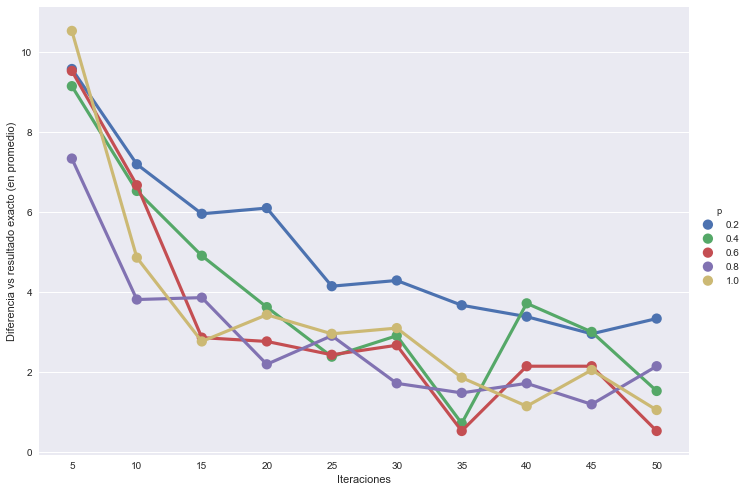
\includegraphics[scale=0.6]{img/grasp-it-v-p.png}
\end{center}

Al ver más de cerca los datos, promediando las diferencias de todos nuestros casos de prueba, podemos observar la variabilidad de nuestro algoritmo: en promedio, nuestras pruebas dieron resultados igual de precisos con $p = 0.6$ realizando 35 o 50 iteraciones. Es más, para ningún valor de p obtuvimos una linea estrictamente decreciente, que sería lo esperable de algorítmos determinísticos.

También podemos ver que en varias ocasiones, para distintas cantidades de iteraciones, otros valores de p dieron resultados más precisos. Sin embargo, consideramos que aumentar la cantidad de iteraciones reduce la variabilidad introducida por las búsquedas golosas aleatorias (porque al iterar siempre conservamos el mejor resultado), por lo que la mayor cantidad de iteraciones es más representativa del valor óptimo de p.
\pagebreak
\section{Heurística constructiva golosa}
\subsection{Introduccion}
Dado que la complejidad del algoritmo exacto resulta prohibitiva en la práctica, podemos aplicar heurísticas que resuelvan el problema en tiempo polinomial, a cuestas de la calidad final de la solución.

Las heurísticas tienen un factor importante de intuición sobre por qué podrían llegar a funcionar mejor o peor y no justificación formal. Debido a esto es difícil decidir qué criterio utilizar puesto que siempre es posible encontrar instancias para las cuales la heurística sea mala.

Nosotros decidimos encarar el criterio de una manera simple y segura, agregar nodos a la clique que nos aumenten la frontera de nuestra clique actual, hasta que no nos queden más aristas por agregar a la clique que nos aumenten la frontera.

\subsection{Desarrollo}
A la hora de aplicar esta heurística sobre nuestro problema, debimos poner el foco sobre donde queríamos realizar la construcción golosa. Rápidamente, y considerando que al utilizar la idea greedy debemos siempre tomar la decisión que mejora nuestra solución de manera óptima a corto plazo (es decir, que dada una clique de tamaño $n$, se obtiene la mejor solución de tamaño $(n+1)$ que contiene a la clique anterior), notamos que la forma acertada de aplicar esta heurística sería, en cada paso, agregar el nodo de mayor grado que genere una clique y mejore la frontera. Es decir que en el primer paso tomaremos siempre al nodo de mayor grado (puesto que esta es la clique de máxima frontera de tamaño 1) y en cada paso le agregaremos el nodo de mayor grado que sea adyacente a toda la clique y que mejore la frontera.

Es importante, antes de seguir, marcar algunas cosas importantes sobre nuestra solución. Para empezar, consideremos que cada vez que agregamos un nodo nuevo a la clique, debemos sumar el grado del nuevo nodo y restar dos veces el tamaño de la subclique (una vez para descontar las aristas que van del nuevo nodo a la clique, y otra para descontar las aristas que iban de cada nodo de la clique al nuevo nodo). Simplificando, tenemos que realizar el siguiente cálculo:

\begin{center}
Para $V_i$ vértice que se agrega a subclique
$Frontera(Clique) = Frontera(Subclique) + d(V_i) - tam(subclique)$ $\times$ $2$
\end{center}

Como vemos, la única variable que cambia cada vez que agregamos un nodo a la clique es el grado del mismo. Por lo tanto, sabemos que si agregar el nodo de mayor grado posible implica empeorar la frontera, entonces todos los nodos de menor grado a él también la empeoraran (lo cual, visto de otra forma, significa también que agregar ese nodo implica tomar la mejor decisión a corto plazo).

Por lo tanto, sabemos que estamos tomando siempre la mejor decisión rápida. Ahora bien, es importante marcar que, llegado el punto en el cual no conseguimos una manera de agrandar la clique mejorando la frontera, la mejor decisión es detenerse. Esto implica no solo que no podemos dar el próximo paso sin achicar la frontera, sino que a partir de este punto no se podrá mejorar la frontera en ningún paso. Esto es fácil de ver si consideramos lo que vimos antes: si el nodo de mayor grado posible empeora la frontera, todos los de grado menor a él también lo hacen. Supongamos que, efectivamente decidimos agregar un nodo $j$ a la clique, de manera que nuestra frontera disminuya, pero luego encontramos un nodo $i$ que podemos agregar a la clique de forma que la frontera crezca. Esto implicará lo siguiente:

\begin{center}
Para $C$ clique original, $C_i$ clique con nodo i, $C_{ij}$ clique con nodos i y j.
$$Frontera(C_i) = Frontera(C) + d(i) - tamano(C) \times 2$$
$$Frontera(C_{ij}) = Frontera(C_i) + d(j) - (tamano(C) + 1) \times 2$$

Vimos que $Frontera(C_{ij})$ $>$ $Frontera(C_i)$, lo cual implica $d(j) > (tamano(C) + 1) \times 2)$, es decir, $d(j) > tamano(C) \times 2$

Pero $Frontera(C_i)$ $<$ $Frontera(C)$, lo cual implica $d(i) < tamano(C) \times 2$

Por lo tanto, tenemos $d(j) > tamano(C) \times 2 > d(i)$, es decir, $d(j) > d(i)$. Pero entonces, eso implica que al agregar el nodo $i$ no agregamos el de mayor grado, puesto que $j$ es adyacente a todos los nodos de $C$ y es de mayor grado que $i$. Absurdo.
\end{center}

De este modo, tenemos una heurística constructiva golosa válida, que toma siempre la mejor decisión posible relacionada al próximo paso y se detiene cuando ya no hay forma de agrandar su frontera agregando nodos a la clique. Considerando entonces este desarrollo, obtenemos el siguiente algoritmo:

\begin{algorithm}[H]
	\NoCaptionOfAlgo
	\caption{\algoritmo{constructivaGolosa}{\In{listaAdyacencia}{lista}}{clique}}

    mayor $\leftarrow$ nodoDeMayorGrado(lista)

    agregarNodoAClique(res, mayor])

    nodosAdyacentes $\leftarrow$ adyacentes(lista, mayor)

    ordenarPorGrado(nodosAdyacentes)

    \For{$i \leftarrow 0$ \KwTo nodosAdyacentes.largo}{
		\If{esAdyacenteATodos(nodosAdyacentes[i], res, listaAdyacencia) $\land$ \\ aumentaLaFrontera(nodosAdyacentes[i], res, listaAdyacencia)}{
			agregarNodoAClique(res, nodosAdyacentes[i])

	}
}
\end{algorithm}

\subsection{Complejidad Temporal}

Esta implementación es bastante sencilla y solo utiliza unas pocas funciones. Veamos la complejidad temporal en peor caso de ellas para después ver la del algoritmo general.

\begin{itemize}
    \item \textbf{nodoDeMayorGrado}: Recorre los n nodos en la lista y se fija el largo de sus adyacentes en $O(1)$ por lo que la función es $O(n)$.

	\item \textbf{ordenarPorGrado}: Esta función utiliza por detrás el sort de la STD, y por ende su complejidad en peor caso es de $O(n*log(n))$. Como sabemos que no recorremos los $n$, sino $|maxAdyacente|$,  podríamos acotarlo por $O(|maxAdyacente|*log(|maxAdyacente|))$

    \item \textbf{esAdyacenteATodos}: Busca si hay un nodo en la clique que no sea adyacente a este nuevo nodo. Para eso, arma un arreglo de booleanos del tamaño del grafo ($O(n)$) y recorre los nodos adyacentes al nodo a insertar (pueden ser hasta $n-1$). Después, basta con recorrer los nodos de la clique y fijarse en el arreglo si son adyacentes o no. Siguiendo este procedimiento, el algoritmo tiene una complejidad temporal $O(n + |adyacentes| + |clique|)$. Es facil ver que $O(|maxClique|)$ $\subseteq$ $O(|maxAdyacentes|)$ , por lo que, si tomamos estas cotas, tendremos $O(n + |adyacentes| + |clique|)$ $\subseteq$ $O(n$ $+ |maxAdyacentes|$ $+ |maxClique|)$ $\subseteq$ $O(n + |maxAdyacentes| + |maxAdyacentes|)$. Veamos, entonces, que $|maxAdyacentes|$ esta acotado por $n - 1$ (puesto que un nodo puede llegar como máximo a todos los nodos del grafo que no son él) por lo que tenemos $O(|maxAdyacentes|)$ $\subseteq$ $O(n)$. Por ende, podemos afirmar $O(n + |maxAdyacentes| + |maxAdyacentes|)$ $\subseteq$ $O(n)$, y nuestra cota queda definida por el costo de armar el vector de booleanos.

    \item \textbf{aumentaLaFrontera}: Hace una simple aritmética entre la cantidad de nodos y la cantidad de adyacentes de la clique por lo que su complejidad es $O(1)$.

    \item \textbf{agregarNodoAClique}: Se encarga de actualizar la clique agregando atrás del vector de nodos en la clique el nodo a insertar en $O(1)$.

\end{itemize}

Ahora analicemos la complejidad de la heurística completa. Inicialmente buscamos el nodo de mayor grado y ordenamos sus adyacentes. Aquí, la operación más costosa es la de ordenar en un tiempo $O(|maxAdyacente|*log (|maxAdyacente|))$. Luego, tomamos el nodo de mayor grado y, para cada uno de sus nodos adyacentes, fijarnos si es posible agregarlo a la clique (es decir, si esAdyacenteATodos). Por lo tanto, para $|maxAdyacente|$ corremos un algoritmo de costo $O(n)$.

Sin embargo, así como vimos que $|maxAdyacente|$ $\leq$ (n - 1), es fácil ver que en un grafo de 40 nodos y 5 aristas, $|maxAdyacente|$ $\leq$ 5 (puesto que un nodo jamás tendrá 6 o más adyacencias, ya que eso implicaría tener 6 o más aristas en el grafo). Por ende, si extendemos esto a todos los grafos, vemos que $O(|maxAdyacente|)$ $\subseteq$ $O(min(n,m))$ , por lo que acabamos teniendo $O(min(n,m))$ $\times$ $O(n)$.

Por ende, al implementar la misma cota sobre ordenarPorGrado, tenemos las siguientes operaciones a considerar: se encuentra el nodo de mayor grado en $O(n)$, se ordena por grado en $O(min(n,m)$ $\times$ $log(min(n,m)))$, y se arma la clique en $O(min(n,m)$ $\times$ $n )$.  Entonces, nuestra cota temporal acaba siendo $O(n + min(n,m)$ $\times$ $log(min(n,m)) + min(n,m)$ $\times$ $n )$. Simplemente, vemos que $O(n)$ $\subseteq$ $O(min(n,m)$ $\times$ $n )$, y como $O(min(n,m))$ $\subseteq$ $O(n)$ (porque siempre $n$ será mayor o igual al mínimo entre $n$ y $m$) , tenemos que $O(min(n,m)$ $\times$ $log(min(n,m)))$ $\subseteq$ $O(min(n,m)$ $\times$ $n )$. Por lo tanto, nuestra cota acaba siendo $O(min(n,m)$ $\times$ $n )$.

\subsection{Casos Patológicos}

La heurística falla en el resultado máximo, cuando uno de los nodos de mayor grado que siguen formando la clique no pertenece a la del resultado esperado, si esto sucede, otros nodos de menor grado nos permiten conseguir en conjunto una mayor frontera.

En la sección de Análisis de precisíón de heurísticas analizaremos más a fondo estos casos, y los compararemos con las otras heurísticas a presentar.

\begin{SCfigure}[1][h]
\caption{En este caso podemos apreciar que si elegimos el nodo de máximo grado(5), esta va a ser nuestra frontera maximal. Pero en cambio la clique formada por los nodos de menor grado(4) en conjunto su frontera es mayor, obteniendo una frontera de 6.}
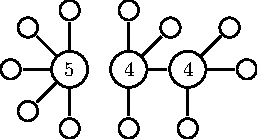
\includegraphics[width=0.5\textwidth]{img/patologic.pdf}
\end{SCfigure}

Podemos generar este tipo de grafos, teniendo una diferencia en el resultado máximo tan grande como queramos. Podemos definir una familia de instancias, que el nodo de mayor grado, digamos de grado k, tal que sus adyacentes son solo adyacentes a él (formando una frontera $k$), a este mismo grafo pertenece una clique de $\frac{k}{2}$ nodos y cada uno de estos además es adyacente a $\frac{k}{2}$ de grado 1. Los nodos de esta clique tienen grado $k - 1$ por lo que en la golosidad hubiésemos preferido el de grado $k$, pero la clique paralelamente construída tiene $\frac{k}{2}$ nodos con $\frac{k}{2}$ adyacentes no pertenecientes a la clique, por lo que la frontera es de $\frac{k}{2} \times \frac{k}{2} = \frac{k^2}{4}$.

Notemos que la diferencia de frontera es de $\frac{k^2}{4} - k$ por lo basta con tomar un $k$ mayor para que la diferencia sea tan grande como queramos, por lo que los grafos con esta particularidad la heurística arrojará malos resultados y estimaciones.

\subsection{Experimentación}

El desafío que nos encontramos al analizar la complejidad de nuestras heurísticas fue que las mismas dependían no solo de $n$ y $m$, sino de la relación entre las mismas (el grado máximo de los nodos). Decidimos estudiar el peor caso en términos de tiempos de ejecución, que es el grafo completo. Por otro lado, consideramos analizar algunos casos promedio, pero el tiempo de ejecución depende de muchos aspectos (grado máximo, tamaño de la clique, etc.), por lo que resultó demasiado difícil medir y analisar estos casos.

\noindent
\begin{minipage}{0.55\textwidth}
    \hfill
    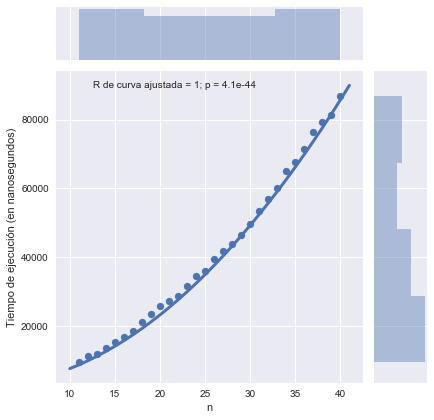
\includegraphics[scale=0.6]{img/greedy-complete.png}
\end{minipage}
\hfill
\begin{minipage}{0.44\textwidth}
    \begin{center}
        Datos del gráfico

        \begin{tabular}{ | l l |}
            \hline
            Grafo completo & $m = \frac{n * (n-1)}{2}$\\ 
            Curva aproximada & $f(x) = 52 * x^2 + 2500$ \\
            \hline
        \end{tabular}
    \end{center}
\end{minipage}

Como se puede observar, nuestra cota teórica de $O(min(n,m)$ $\times$ $n)$ aplica correctamente para nuestro peor caso. En este contexto, n siempre es menor a m, por lo que $O(min(n,m)$ $\times$ $n) = O(n^2) = O(m)$. Podemos analizar esto mismo graficando los mismos datos en funcion de m:

\noindent
\begin{minipage}{0.55\textwidth}
    \hfill
    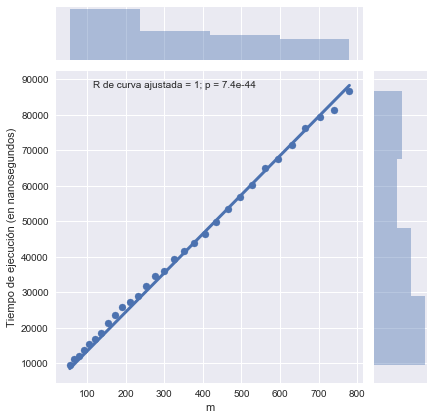
\includegraphics[scale=0.6]{img/greedy-complete-m.png}
\end{minipage}
\hfill
\begin{minipage}{0.44\textwidth}
    \begin{center}
        Datos del gráfico

        \begin{tabular}{ | l l |}
            \hline
            Grafo completo & $m = \frac{n * (n-1)}{2}$\\ 
            Curva aproximada & $f(x) = 110 * x + 2500$ \\
            \hline
        \end{tabular}
    \end{center}
\end{minipage}

Cabe reiterar que esto solo aplica en nuestro contexto de grafo completo. El tiempo de ejecución puede variar de forma distinta si no se tienen encuenta los factores anteriormente mencionados, como el grado máximo o el tamaño de la clique máxima del grafo.


% LALALALALA MALDITO CASO PROMEDIO
% Para analizar el caso general, utilizamos dos estrategias distintas para la generación automática de los grafos:

% \begin{itemize}
%     \item uniforme: se generan grafos con ejes aleatorios, basandose en un grafo completo y utilizando una distribución uniforme para remover aristas excedentes

%     \item grado máximo: en este caso se parte de un nodo de grado máximo y se agregan adyacencias de forma ordenada, siempre evitando exceder el grado máximo preestablecido
% \end{itemize}

% Ambas estrategias presentan sus ventajas y desventajas: la generación uniforme solo permite analizar n y m de manera independiente, lo cual dificulta el análisis, mientras que la generación por grado máximo puede dar casos sesgados ya que los ejes no están apropiadamente distribuidos, y pueden dar casos particularmente favorables o desfavorables para la heurística.

% \subsubsection*{Grafos uniformes}

% \noindent
% \begin{minipage}{0.49\textwidth}
%     \hfill
%     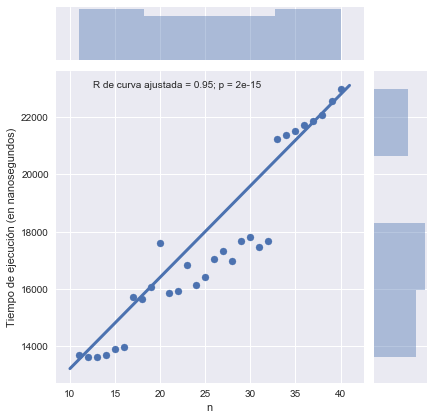
\includegraphics[scale=0.55]{img/greedy-n-low.png}

%     \begin{center}
%         Datos del gráfico

%         \begin{tabular}{ | l l |}
%             \hline
%              & $m = 40$ \\ 
%             \hline
%         \end{tabular}
%     \end{center}
% \end{minipage}
% \hfill
% \begin{minipage}{0.49\textwidth}
%     \hfill
%     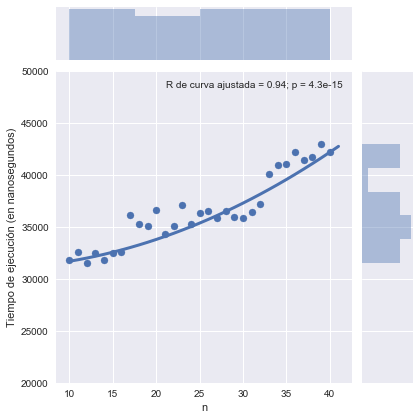
\includegraphics[scale=0.55]{img/greedy-n-hi.png}

%     \begin{center}
%         Datos del gráfico

%         \begin{tabular}{ | l l |}
%             \hline
%              & $m = 20$ \\
%             \hline
%         \end{tabular}
%     \end{center}
% \end{minipage}

% Nuestros primeros experimentos nos dejaron muy sorprendidos: en casos promedio, si aislamos n, pareciese tener una relación inversa con el tiempo de ejecución mientras n < m, pero no influye una vez que n > m.

% Si bien no aproximamos ninguna curva, utilizamos el coeficiente de correlacion de Spearman para analizar estos resultados. El mismo sirve para detectar correlaciones no necesariamente lineales o uniformemente distribuídas, pero sí monótonas (es decir, estrictamente positivas o negativas).


% \noindent
% \begin{minipage}{0.49\textwidth}
%     \hfill
%     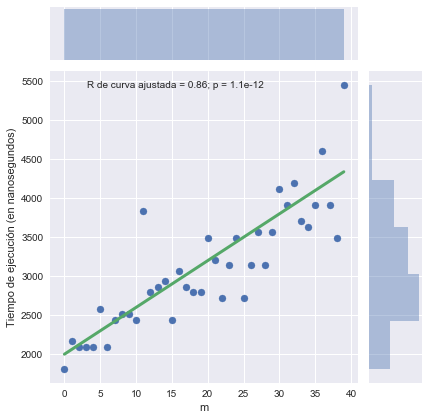
\includegraphics[scale=0.55]{img/greedy-m-low.png}

%     \begin{center}
%         Datos del gráfico

%         \begin{tabular}{ | l l |}
%             \hline
%              & $n = 40$ \\
%             Curva aproximada & $f(x) = 60 * x + 2000$ \\
%             \hline
%         \end{tabular}
%     \end{center}
% \end{minipage}
% \hfill
% \begin{minipage}{0.49\textwidth}
%     \hfill
%     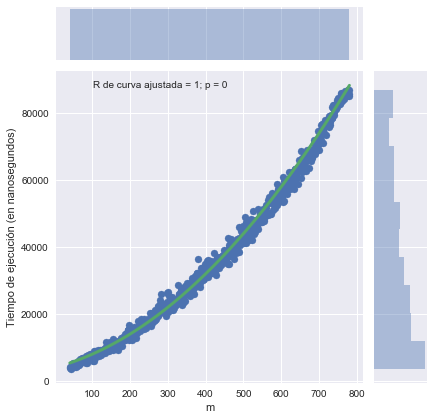
\includegraphics[scale=0.55]{img/greedy-m-hi.png}

%     \begin{center}
%         Datos del gráfico

%         \begin{tabular}{ | l l |}
%             \hline
%              & $n = 40$ \\
%             Curva aproximada & $f(x) = \frac{x^2}{10} * 30 * x + 4000$ \\
%             \hline
%         \end{tabular}
%     \end{center}
% \end{minipage}

% Al hacer un análisis similar en base a m, nos encontramos que un aumento en m derivaba indefectiblemente en un aumento del tiempo de ejecución. En particular, parecería que si m > n, el algorítmo ejecuta en $O(m^2)$.

% Nuestra conclusión ante estos resultados fue que las cotas de complejidad propuestas no necesariamente son incorrectas, pero al no poder garantizar el valor del factor determinante (el máximo grado del grafo) estos resultan engañosos, ya que existe una relación positiva entre el grado de los nodos y la cantidad de ejes, mientras que existe una relación inversa entre la cantidad de nodos y sus grados, asumiendo que los ejes están distribuídos de manera uniforme.

% \subsubsection*{Grafos con grado máximo}

% Para suplir las falencias de los datos uniformes, decidimos analizar grafos con grados máximos garantizados, al costo de perder la distribución uniforme de sus ejes.

% Si bien consideramos que es posible generar grafos que cumplan con ambos requisitos, el esfuerzo involucrado es mayor, por lo que decidimos no incluir dicho análisis en el presente trabajo.

% \noindent
% \begin{minipage}{0.55\textwidth}
%     \hfill
%     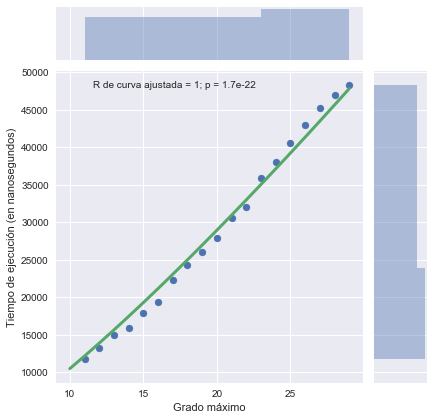
\includegraphics[scale=0.6]{img/greedy-alt-maxdeg.png}
% \end{minipage}
% \hfill
% \begin{minipage}{0.44\textwidth}
%     \begin{center}
%         Datos del gráfico

%         \begin{tabular}{ | l l |}
%             \hline
%              & $n = 20$\\ 
%             Curva aproximada & $f(x) = 580 * x + 10000$ \\
%             \hline
%         \end{tabular}
%     \end{center}
% \end{minipage}

% Por otro lado, el impacto lineal de la cantidad de aristas fue más que evidente. Debido a la superposición de los puntos, la curva aproximada debió ser graficada en otro color.



% compilar 2 veces para actualizar las referencias


\end{document}